%version of 11-28-18

\chapter{COMBINATORICS, PROBABILITY, AND STATISTICS}
\label{ch:combinatorics}

\section{Combinatorial interpretation of Fibonacci numbers}

Let us count the number of binary vectors whose components donot have two
consecutive $1$. Call $F(n)$ this number.

Look at the last bit of the binary representation of $n$.

\begin{itemize}
\item
If it is equal to $1$ thus, the previous bit (in position $n-1$ should be $0$.
In this first case, the number the number is equal to $F(n-2)$
\item
If the last bit is $0$, the number is $F(n-1)$
\end{itemize}
Thus, $F(n) = F(n-1) + F(n-2)$
\bigskip

This alternative view of looking at the Fibonacci numbers allows us to establish some elegant proofs.
This is for instance the case for Property~\ref{thm:FiboSum-1}. 



\section{The Fundamentals of Counting}
\label{sec:counting}


\subsection{Binary Strings and Power Sets}

\begin{prop}
\label{thm:b-ary strings}
For every integer $b > 1$, there are $b^n$ $b$-ary strings of length
$n$.
\end{prop}

\begin{proof}
The asserted numeration follows most simply by noting that there are
always $b$ times as many $b$-ary strings of length $n$ as there are of
length $n-1$.  This is because we can form the set of $b$-ary strings
of length $n$ as follows.  Take the set $A_{n-1}$ of $b$-ary strings
of length $n-1$, and make $b$ copies of it, call them $A^{(0)}_{n-1},
A^{(1)}_{n-1}, \ldots, A^{(b-1)}_{n-1}$.  Now, append $0$ to every
string in $A^{(0)}_{n-1}$, append $1$ to every string in
$A^{(1)}_{n-1}$, \ldots, append $\bar{b} = b-1$ to every string in
$A^{(b-1)}_{n-1}$.  The thus-amended sets $A^{(i)}_{n-1}$ are mutually
disjoint (because of the terminal letters of their respective
strings), and they collectively contain all $b$-ary strings of length
$n$.  \qed
\end{proof}

\medskip

\addcontentsline{toc}{subsubsection}{-- A fun result: $n$-element sets
  have $2^n$ subsets}

\begin{prop}
\label{thm:power-sets}
The power set $\p(S)$ of a finite set $S$ contain $2^{|S|}$ elements.
\end{prop}

\begin{proof}
Let us begin by taking an arbitrary finite set $S$---say of $n$
elements---and laying its elements out in a line.  We thereby
establish a correspondence between $S$'s elements and positive
integers: there is the first element, which we associate with the
integer $1$, the second element, which we associate with the integer
$2$, and so on, until the last element along the line gets associated
with the integer $n$.

Next, let's note that we can specify any subset $S'$ of $S$ by
specifying a length-$n$ {\em binary (i.e., base-$2$) string}, i.e., a
string of $0$'s and $1$'s.  The translation is as follows.  If an
element $s$ of $S$ appears in the subset $S'$, then we look at the
integer we have associated with $s$ (via our linearization of $S$),
and we set the corresponding bit-position of our binary string to $1$;
otherwise, we set this bit-position to $0$.  In this way, we get a
distinct subset of $S$ for each distinct binary string, and a distinct
binary string for each distinct subset of $S$.

Let us pause to illustrate our correspondence between sets and strings
by focussing on the set $S = \{a,b,c\}$.  Just to make life more
interesting, let us lay $S$'s elements out in the order $b,a,c$, so
that $b$ has associated integer $1$, $a$ has associated integer $2$,
and $c$ has associated integer $3$.  We depict the elements of $\p(S)$
and the corresponding binary strings in the following table.
\begin{center}
\fbox{
\begin{tabular}{c|c|c}
Binary string & Set of integers & Subset of $S$ \\
\hline
$000$ & $\emptyset$ & $\emptyset$ \\
$001$ & $\{3\}$     & $\{c\}$ \\
$010$ & $\{2\}$     & $\{a\}$ \\
$011$ & $\{2,3\}$   & $\{a,c\}$ \\
$100$ & $\{1\}$     & $\{b\}$ \\
$101$ & $\{1,3\}$   & $\{b,c\}$ \\
$110$ & $\{1,2\}$   & $\{a,b\}$ \\
$111$ & $\{1,2,3\}$ & $\{a,b,c\} =S$
\end{tabular}
}
\end{center}

Back to the Proposition: We have verified the following: {\em The
  number of length-$n$ binary strings is the same as the number of
  elements in the power set of $S$!}  The desired numeration thus
follows by the ($b=2$) instance of Proposition~\ref{thm:b-ary
  strings}.  \qed
\end{proof}

\begin{quote}
The binary string that we have constructed to represent each set of
integers $N \subseteq \{0, 1, \ldots, n-1\}$ is called the {\it
(length-$n$) characteristic vector}\index{characteristic vector}
{\it of the set} $N$.  Of course, the finite set $N$ has
characteristic vectors of all finite lengths.  Generalizing this idea,
{\em every} set of integers $N \subseteq \N$, whether finite or
infinite, has an {\em infinite} characteristic vector, which is formed
in precisely the same way as are finite characteristic vectors, but
now using the set $\N$ as the base set.
\end{quote}


\section{The Elements of Probability}
\label{ch:prob-stat}



 within discrete frameworks, including introducing
discrete probability/likelihood as a ratio:
\[ 
\frac{\mbox{number of targeted events}}{\mbox{number of possible events}}
\]


Elements of probability theory and statistics infuse every area of
computing.  The practicality of many algorithms that are
experientially the most efficient for their target tasks depend on the
{\em distribution} of inputs in ``real" situations.  Design
methodologies for crucial complex circuits must acknowledge the {\em
  mean times to failure} of the critical components of the circuits.
Sophisticated searching algorithms must take into account the relative
{\em likelihoods} of finding one's goal in the various optional search
directions.  Analyzing and understanding large corpora of data
requires a variety of methodologies that build on the concepts of {\em
  clustering} and/or {\em decomposition}.

A student needs at least an introduction to the foundations of
probability and statistics to even understand, all the moreso to
master, the terms highlighted in the preceding paragraph.  We outline
many of the key concepts that a student must be exposed to in the
following subsections.


\subsection{The Basic Elements of Combinatorial Probability}

Perhaps the easiest and most engaging way to introduce ``probability
via counting" is by calculating the comparative likelihoods of various
deals in $5$-card poker and of various rolls of a pair of dice.  The
arithmetic required for this discussion is elementary and the
``application" to gambling of interest even to non-gamblers: ``Why is
such a deal in poker (say, a straight) worth more than another (say,
three of a kind)?"  One can also introduce in this setting concepts
such as randomness, bias, etc., that are so important in the design of
experiments and the analysis of their outcomes.

\section{The Token Game}
\label{sec:TokenGame}

\subsection{Principle}

%Let us start by studying a puzzle whose solution can be obtained by a recursive algorithm. 

Consider a bank with $n$ circle positions numbered from $1$ to $n$ and $n$ tokens.
Initially, the bank is empty (see Figure~\ref{fig:jeujetonsInit}).
%\begin{itemize}
%\item Put a token in position $1$ if it is empty or remove the token in position $1$.
%\item Put a token in the position 
%\end{itemize}

\begin{figure}[h]
\begin{center}
        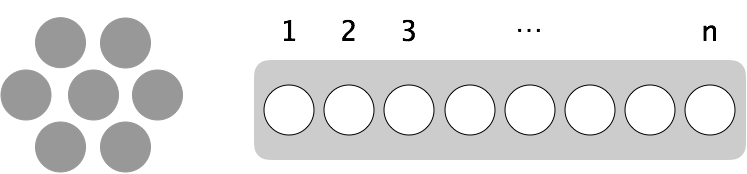
\includegraphics[scale=0.4]{FiguresMaths/GameTokenInit.png}
        \caption{Initial position: $n$ tokens (grey) and all the empty bank.}
        \label{fig:jeujetonsInit}
\end{center}
\end{figure}

The game consists in determining the process to fill the bank with the $n$ tokens, putting or removing one token at a time according to one of the two 
following constraints.
Both rules are illustrated in figures~\ref{fig:rule1} and \ref{fig:rule2}.

\begin{itemize}
\item \textbf{Rule 1.} Position 1: Put a token if it is empty or remove it.
\item \textbf{Rule 2.} Position next to the first empty position (i.e. on the right): Put a token if the position is empty or remove it.
\end{itemize}

Notice that the first rule only refers to positions (and thus, it is symmetric in regard to the move: put or remove a token), 
while the second one is not symmetric.

\begin{figure}[h]
\begin{center}
        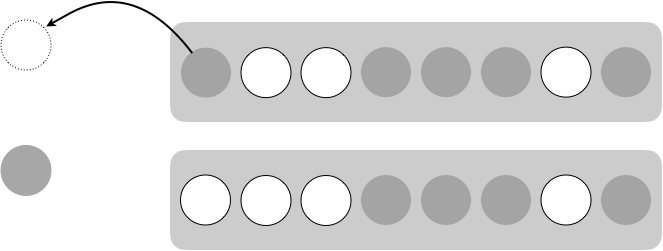
\includegraphics[scale=0.4]{FiguresMaths/GameTokenRule1.png}
        \caption{Rule 1: Position 1 contains a token, thus, remove it.}
        \label{fig:rule1}
\end{center}
\end{figure}

\begin{figure}[h]
\begin{center}
        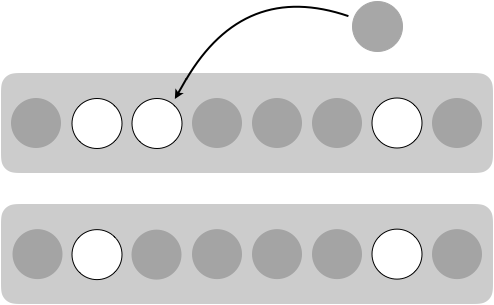
\includegraphics[scale=0.4]{FiguresMaths/GameTokenRule2.png}
        \caption{Rule 2: The position next to the first idle position (i.e. position 3 in this example) 
        is idle, thus, put a remaining token here.}
        \label{fig:rule2}
\end{center}
\end{figure}

The analysis of the game for some particular values of $n$ leads to some evidences (looking at the first ranks):
First, in the even case, the process should start by putting the second token while in the odd case, we should start to fill the first position.
%Then, the first token is flipped every double steps, the second one every four steps and so on.
Second observation: both rules are applied alternatively (this is obvious for Rule 1 since applying it twice consecutively leads to the initial position, 
and easy to check for Rule 2 on the first ranks). 
However, the solution is not easy to describe and its cost is not easy to establish.

The solution can be easily expressed recursively as follows (for $n > 2$):
the token in the last position can only be put bu rule 2, that means that the first $(n-2)$ one are on the bank.
Then, if we empty these first $n-2$ positions,
we obtain a configuration similar as in the initial one except for the last position which has a token. 
Then, the puzzle is solved by applying the same process on a bank with $n-1$ tokens.
The successive steps of this recursive solution are depicted in Figure~\ref{fig:jeujetonsPrinciple}.

%Thus, flipping the first tokens of the same color is different if they are all blue or red.
%Notice that flipping the first reds can be obtained using the reverse process as for the blue ones (see coding at the end of this document).

\begin{figure}[h]
\begin{center}
        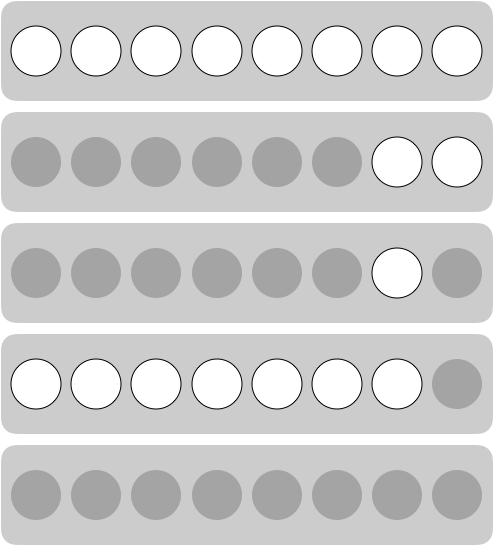
\includegraphics[scale=0.4]{FiguresMaths/GameTokenPrinciple.png}
        \caption{Principle of the recursive solution. Fill the bank in the $(n-2)$ first positions, then, put a token on the last position (Rule 2), 
        empty the (n-2) first positions. Finally, fill the $(n-1)$ first positions of the bank.}
        \label{fig:jeujetonsPrinciple}
\end{center}
\end{figure}
\bigskip

More formally,
\bigskip

fillBank(n)
\begin{itemize}
\item
 if $n=1$ then putToken(1) -- according to Rule 1
\item
if $n=2$ then PutToken(2) -- Rule 2 -- and then PutToken(1) -- Rule 1

\item 
if $n > 2$ then
\begin{itemize}
\item fillBank(n-2)
\item PutToken(n)
\item EmptyBank(n-2)
\item FillBank(n-1)
\end{itemize}
\end{itemize}

\subsection{Analysis}

The analysis comes directly from the previous process. 

Let call $f(i)$ the cost for filling the bank from position $1$ to position $i$
(the cost here refers to the number of elementary moves, put or remove a token).
Notice that it requires the same number of steps to fill or to empty the truncated bank (from position $1$ to $i$). 
The total cost is to fill the whole bank of size $n$, thus we have to solve:

$f(n) = f(n-2) + 1 + f(n-2) + f(n-1) = f(n-1) + 2.f(n-2) +1$ for $n > 2$

with $f(1) = 1$ and $f(2) = 2$.
\bigskip

If we add $f(n-1)$ in both sides of the previous expression, we obtain a simpler equation (call $s(n)$ the sum $f(n)+f(n-1)$ $n \geq 2$,
in particular, $s(2) = 2+1$):

$f(n) + f(n-1) = 2.f(n-1) + 2.f(n-2) +1$

$s(n) = 2.s(n-1)+1 = 2.(2.s(n-2)+1) + 1 = 2^2 s(n-2) + 2+ 1 = 2^3 s(n-3) + 2^2 + 2 + 1 = ... = 2^{n-2} s(2) + 2^{n-3} + ... + 2^2 + 2 + 1$ where $s(2) = 2+1$

$s(n) = 2^{n-1} + 2^{n-2} + 2^{n-3} + ... + 2^2 + 2 + 1$ 

Summing up this geometric series leads to
$s(n) = 2^{n} -1$
\bigskip

Coming back to the $f(n)$, we can rewrite this equation as:

$f(n) = 2^{n} - f(n-1) -1$ where $f(1)=1$

$f(n) = 2^{n} - 2^{n-1} + f(n-2) +1 -1 = 2^{n} - 2^{n-1} + 2^{n-2} - f(n-3) -1 = ...$

This sequence is an alternate series of the powers of $2$ where the $1$ and $-1$ are cancelled two by two.
However, there is a different number of steps if $n$ is even or not. 
In this case, the last term is $-2$, while it is $-1$ when $n$ is odd.
\bigskip

For $n$ even, $f(n) = \sum_{1 \leq k \leq n}(-1)^{k}2^{k} $

For $n$ odd, $f(n) = \sum_{0 \leq k \leq n}(-1)^{k+1}2^{k} $
\bigskip

$f(n)$ is an alternate series of the successive powers of $2$, which can be solved by a graphical proof.

We rewrite it by gathering the positive and negative terms as follows (for odd $n$): 
$f(n) = (2^{n} + 2^{n-2} + ... + 2) - (2^{n-1} + 2^{n-3} + ... + 1)$

$= 2.(2^{n-1} + 2^{n-3}  + ...  +1) - (2^{n-1} + 2^{n-3}  + ... + 1)$

$= 2^{n-1} + 2^{n-3}  + ...  +1$ 

Consider first the odd case (here, $2^{n+1}$ is a perfect square).
Figure~\ref{fig:alternatePowers2odd} gives a representation of $f(n)$ 
where the smallest surface at the right is the unit square.

Take 3 copies of $f(n)$ as it is depicted in figure~\ref{fig:alternatePowers2finalOdd},
two are mirror configurations and the third one (represented in grey) fills the remaining part of a big square but some idle space at the 2 extreme right corners. 
The whole surface is a perfect $2^{n} \times 2^{n}$ square, equal to $2^{n+1}$ plus the small surface equal to half of the basic unit square ($2 \times \frac{1}{2}$ = 1). Thus, $3.f(n)+1= 2^{n+1}$.

\begin{figure} [h]
\begin{center}
        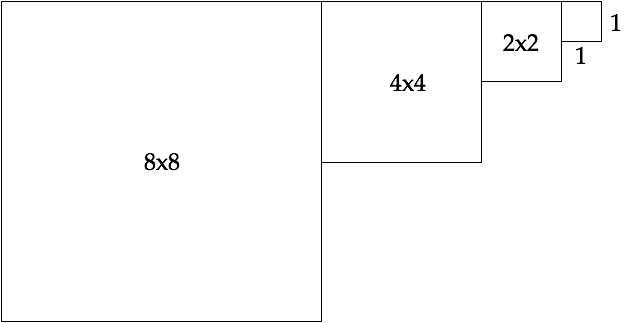
\includegraphics[scale=0.4]{FiguresMaths/alternatePowers2initOdd.png}
        \caption{Representation of the alternate series of powers of $2$ for $n=7$.
        f(7)=64+16+4+1.}
        \label{fig:alternatePowers2odd}
\end{center}
\end{figure}

\begin{figure} [h]
\begin{center}
        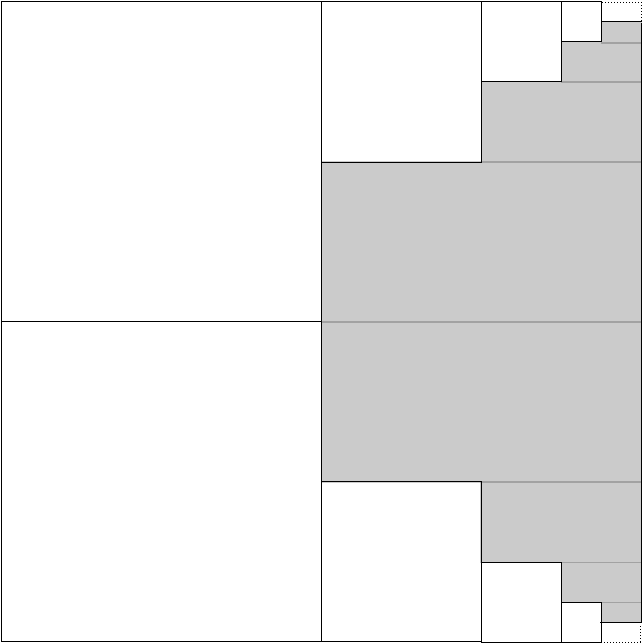
\includegraphics[scale=0.4]{FiguresMaths/alternatePowers2odd.png}
        \caption{Even case: Geometric proof using 3 copies of $f(n)$ that almost fill a large square.}
        \label{fig:alternatePowers2finalOdd}
\end{center}
\end{figure}

The previous construction may be adapted in the even case in a similar way.
The details are left to the readers. 

We propose below another proof obtained by using the results for the odd case:

We start by the expression $f(n) + f(n-1) = 2^n -1$
that is $f(2k) = 2^{2k} - f(2k-1) -1$ for even $n=2k$.

Now, apply the final expression of $f$ to $2k-1$, which is odd: $f(2k-1) = \frac{1}{3} (2^{2k+1}-1)$.

$f(2k) = 2^{2k} - \frac{1}{3} (2^{2k-1+1}-1) -1 = 2^{2k} (1-\frac{1}{3}) + \frac{1}{3} -1= \frac{1}{3} (2^{2k+1} -2)$.
\bigskip

%
%Figures~\ref{fig:alternatePowers2even} and~\ref{fig:alternatePowers2finalEven} illustrate the construction in the even case.
%The details are left to the readers. 
%We obtain $3.f(n)+2= 2^{n+1}$ by a similar analysis.
%However, we can deduce directly the even case from the odd case by remarking that $f(2k)=2.f(2k-1) +1$.
%
%This is obtained by the basic relations $f(n) = 2^{n} - f(n-1) -1$ and $f(2k-1) = \frac{1}{3} (2^{2k} -1)$.
%
%$n=2k$, $f(n) = 2^{2k} - \frac{1}{3} (2^{2k} -1) -1 = \frac{1}{3} (2^{n+1} -2)$.
%
%\begin{figure} [h]
%\begin{center}
%        \includegraphics[scale=0.4]{FIGmaths/alternatePowers2initEven.png}
%        \caption{Representation of the alternate series of powers of $2$ for $n=6$.
%        f(6)=32+8+2.}
%        \label{fig:alternatePowers2even}
%\end{center}
%\end{figure}
%
%
%\begin{figure} [h]
%\begin{center}
%        \includegraphics[scale=0.4]{FIGmaths/alternatePowers2even.png}
%        \caption{Case odd: Geometric proof in the odd case. Notice here that there are 2 small rectangles left at the extreme corners on the right,
%        whose surface is $1$ each.}
%        \label{fig:alternatePowers2finalEven}
%\end{center}
%\end{figure}

We finally obtain: 

$f(n) = \frac{1}{3} (2^{n+1} -1)$ if $n$ is odd.

$f(n) = \frac{1}{3} (2^{n+1} -2)$ if $n$ is even.



\section{Toward a Basic Understanding of Statistics}

Most students whose interest tend to the empirical will likely ``do"
statistics with the aid of apps, rather than by explicitly writing
programs that perform the required calculations.  That said, all
students should understand the crucial notion of {\em random variable}
and should be conversant with the most common statistical
distributions.  ``Conversant" in this context should include complete
understandings of the (low-numbered) moments of {\em at least} the
{\em uniform} and {\em exponential} distributions.  They should know
how to compute, say, the means and variances of various distributions
— and, most importantly, they should {\em understand} the sense in
which the variance of a distribution give {\em important} information
that is not available from the mean.  All of this is prerequisite to
rigor in experimentation.

\subsubsection{The Elements of Empirical Reasoning}

Empirical reasoning does not convey the certitude that formal
reasoning does.  Students should understand how to craft experiments
in a way that collects the ``right'' data.  The should then be
able---perhaps just with statistical packages---to interpret the
results they collect and to understand what conclusions are
justifiable.  {\em It is essential that all students understand the                  
  ditinction between {\em positive correlation} and {\em causation}!}
(Most of the public would seem to flunk that test.)

In order to satisfy the preceding demands, students should understand
enough about statistics---including definitions and meanings related
to distributions and their moments---to understand what conclusions
can be made based on experimental results, and to understand how to
describe conclusions in a way that is supported by the statistics.

\section{Beyond the Basics}

As students are introduced to modern topics within computing, whether
at the level of a Computing Literacy course or a post-core technical
course, they will have to master a variety of more specialized topics
that combine pieces of the elements we have discussed in this essay.
While these topics are beyond the level of generality aimed at in this
essay, some may be appropriate prerequisites to programs that have
some specialized foci.
\begin{itemize}
\item
Issues relating to {\em clustering} find application in applicatios as
diverse as: {\em linear-algebraic computations}, {\em data mining},
{\em design and layout of digital circuitry}.

\item
Issues building on {\em graph separation/decomposition} are
encountered when studying: {\em linear-algebraic computing}, {\em
  fault-tolerant design}, {\em load balancing}.

\item
Many issues relating to {\em fault/failure tolerance} and {\em data
  analytics} benefit from study using {\em random walks} (at least in
one dimension).

\item
Many useful ideas regarding the {\em encoding and manipulation of
  data} can be gleaned from the elements of {\em information theory}
and {\em computer arithmetic}.
\end{itemize}
The preceding list is really endless.  Hopefully readers will be
inspired by our few examples to compile a longer version that is
appropriate for their particular environments.




